\documentclass{article}
\usepackage[utf8]{inputenc}
\usepackage{amsfonts}
\usepackage{algorithm2e}
\usepackage{amsmath}
\usepackage[a4paper]{geometry}
\geometry{hscale=0.8,vscale=0.9,centering}
\usepackage{graphicx}
\usepackage{program}
\usepackage{ulem}
\usepackage{xcolor}
\usepackage{pdfpages}
\usepackage{hyperref}
\newcommand{\subsubsubsection}[1]{\paragraph{#1}\mbox{}\\}
\setcounter{secnumdepth}{4}
\setcounter{tocdepth}{4}
\newcommand{\alinea}{
\textbf{\hspace{8mm}}
}
 \setlength{\parindent}{0pt}
 
\newcommand{\sautligne}{
\textbf{\vspace{5mm}}
}



\title{M1 Info – ARC - LAB4}
\author{Olivier HUREAU - Groupe 3}
\date{25/03/2020}

\begin{document}
\maketitle
\renewcommand{\contentsname}{Table des matières}
\tableofcontents
\newpage

\section{Évaluation de la qualité des tests.}
Les différents types de couverture nous intéréssant sont 
\begin{itemize}
	\item State / Transition coverage : En principe les testbench vérifie que la machine passe dans tout les états. Si nous n'avons pas 100\% de couverture ici c'est qu'il y a un problème.
		\item Branch coverage : Si le teste de couverture remonte des erreurs, il sera alors plus facile de traquer les erreurs de transissions..
	\item Statement coverage : Les statements influant sur les branchements, ce test de couverture nous permet aussi de vérifier le comportement du robot.

\end{itemize}

Les tests "line coverage" et  donne une indication sur la présentation ou l'optimisation du code, ne nous souciants uniquement du bon fonctionnement de notre implémentation, il ne nous sont pas utiles.

Le test Toggle coverage donnant une indication sur la robustesse du l'implémentation. Il est bien trop compliqué et trop long d'analyser les résultats de ce test dans le cadre de nos labs.


\subsection{Première analyse}

\subsubsection{Résultats du test de coverage}

\paragraph{Résultats du test de coverage sur le système entier}

Ci dessous : S est l'architecture System, C1 et C2 les compteurs et R le robots dans le testbench System.
\begin{figure}[!h]
\advance\leftskip+3cm
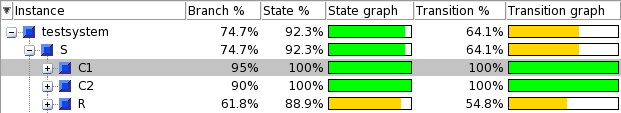
\includegraphics[scale=0.70]{PremiereAnalyse/Coverage.PNG}
\caption{Résultats de couverture Branch, State et Transition sur le système entier}
\end{figure}

Le graph de couverture du robot dans le testbench system

\begin{figure}[!h]
\advance\leftskip+3cm
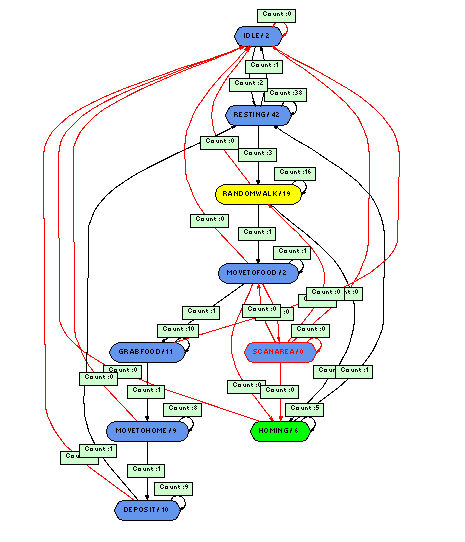
\includegraphics[scale=0.80]{PremiereAnalyse/graph.PNG}
\caption{Graph de couverture d'état sur le système entier}
\end{figure}

\paragraph{Résultats du test de coverage sur le robot}

Ci dessous : S est l'architecture System, C1 et C2 les compteurs et R le robots dans le testbench System.
\begin{figure}[!h]
\advance\leftskip+3cm
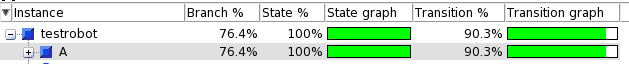
\includegraphics[scale=0.70]{PremiereAnalyse/coverRobot.PNG}
\caption{Résultats de couverture Branch, State et Transition sur le robot}
\end{figure}

Le graph de couverture du robot dans le testbench system

\begin{figure}[!h]
\advance\leftskip+3cm
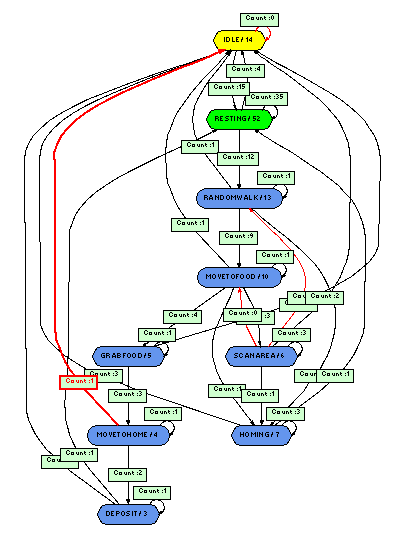
\includegraphics[scale=0.65]{PremiereAnalyse/graphRobot.PNG}
\caption{Graph de couverture d'état sur le robot}
\label{graphe-robot}
\end{figure}.



On observera aussi le code coverage analysis :

\begin{figure}[!h]
\advance\leftskip+3cm
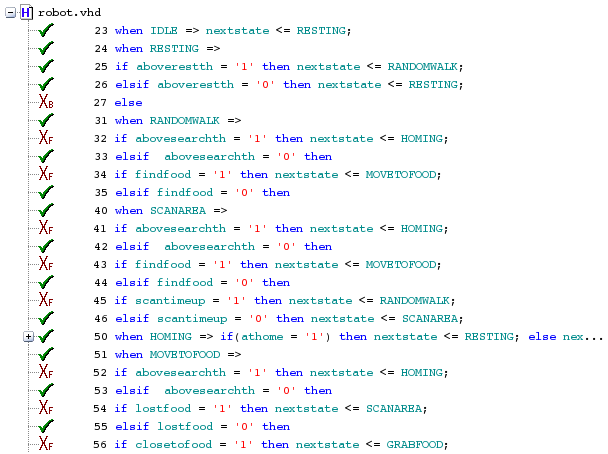
\includegraphics[scale=0.7]{PremiereAnalyse/codeCov.PNG}
\caption{Graph de couverture d'état sur le robot}

\end{figure}


\paragraph{Interprétation des résultats}
Les tests de couverture sont très probant (87\% pour le système entier). Cependants, on vois que des dans le système entier, l'état SCANAREA n'est jamais atteins bien que les tests de système (se reporter au tableau du précédent lab) avais prévu un chemin pour arriver jusqu'à cet état ainsi que d'utiliser ses transitions. 

L'analyse du robot avec un testbench différent nous donne alors des indications suivantes : certaines transitions ne sont jamais atteintes, l'état SCANAREA est bien accessible pour l'automate. 
\sautligne

Deux hyptohèses se posent alors : Soit le système est mal conçus, soit c'est les testbenchs. Avant de se replonger dans le une éventuelle réécriture des architectures et/ou entité (la couverture des branch pourrons nous aider pour cela). Il faut être certains que c'est les testbenchs qui ne sont pas faux.

Après interprétation des résultats, on créer des séquences de signaux qui nous permettrons d'être sur que le testbenchs du robot n'est pas faux.



\subsection{Correction du code après une première analyse }

\subsubsection{Correction du testbench du robot}

\paragraph{Les branchements}

Le code coverage analysis nous indique que certains branchement ne sont pas excuté. En effet, j'avais mis des sécurités sur mes conditions. Prennons l'exemple suivant : .

\begin{verbatim}
if aboverestth = '1' then nextstate <= RANDOMWALK;
elsif aboverestth = '0' then nextstate <= RESTING;
\end{verbatim} 

Je voulais être sur que le deuxième statement ne s'execute uniquement si aboverestth vaut '0' et non pas si aboverestth est différent de '1'.

Je ne sais pas si je dois garder cette sécurité.. Pour les tests de couverture, je l'enlève donc.

\sautligne

\paragraph{Les etats et les transitions}
Grace au graph de couverture (figure \ref{graphe-robot}) il faut tester les transitions suivantes :
\begin{itemize}
\item Reset depuis MOVETOHOME
\item Aller de SCANAREA à MOVETOFOOD (rappel de contraintes de transition : Aboveseartch ='0' \& findfood = '0' \& scantimeup = '1')
\item Aller de SCANAREA à RANDOMWALK (rappel de contraintes de transition : Aboveseartch ='0' \& findfood = '1' )
\end{itemize}

\paragraph{Résultat après correction}
Après correction, on obtiens donc les résultats suivants :

\begin{verbatim}
Coverage Report Summary Data by file

=================================================================================
=== File: /tp/xm1iarc/xm1iarc003/projet_asic/ARC/lab4/robot.vhd
=================================================================================
    Enabled Coverage            Active      Hits    Misses % Covered
    ----------------            ------      ----    ------ ---------
    Stmts                           28        28         0     100.0
    Branches                        43        43         0     100.0
    FEC Condition Terms             11        11         0     100.0
    FSMs                                                       100.0
        States                       9         9         0     100.0
        Transitions                 31        31         0     100.0

=================================================================================
=== File: /tp/xm1iarc/xm1iarc003/projet_asic/ARC/lab4/testRobot.vhd
=================================================================================
    Enabled Coverage            Active      Hits    Misses % Covered
    ----------------            ------      ----    ------ ---------
    Stmts                           14        14         0     100.0


Total Coverage By File (code coverage only, filtered view): 100.0%
\end{verbatim}

\begin{figure}[!h]
\advance\leftskip+3cm
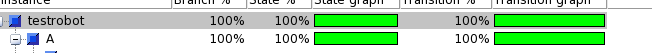
\includegraphics[scale=0.7]{PremiereCorrection/resultats.PNG}
\caption{Rapport de couverture}

\end{figure}

\paragraph{Conclusion de la correction du robot}
Avec ces tests de couvertures qui dont concluant, on peux donc affirmer que le robot se comporte correctement grâce au modifications effectué sur notre code.

Voir annexes : 

\subsubsection{Correction du testbench du system}

On sait ici que plusieurs problèmes sont à résoudre pour obtenir un test de couverture concluant. Il faut donc : 
\begin{itemize}
\item Passer dans l'état SCANAREA
\item Utiliser les différentes transitions :
	\begin{itemize}
	\item MOVETOFOOD vers SCANAREA (Contraines : abovesearchth = '0' \& losftood = '1' )
	\item SCANAREA vers RANDOMWALK (Contraines: abovesearchth = '0' \& findfood = '0' \& scantimeup = '1'  )
	\item SCANAREA vers MOVETOFOOD (Contraines : abovesearchth = '0' \& findfood = '1' )
	\item SCANAREA vers HOMING (Contraines : abovesearchth ='1' )
	\end{itemize}
\item Utiliser le reset dans pour tout les états
\end{itemize}

\paragraph{Résultat après correction}
Après correction, on obtiens donc les résultats suivants :
\begin{verbatim}
Coverage Report Summary Data by file

=================================================================================
=== File: /tp/xm1iarc/xm1iarc003/projet_asic/ARC/lab4/count.vhd
=================================================================================
    Enabled Coverage            Active      Hits    Misses % Covered
    ----------------            ------      ----    ------ ---------
    Stmts                           17        17         0     100.0
    Branches                        20        19         1      95.0
    FEC Condition Terms             10         6         4      60.0
    FSMs                                                       100.0
        States                       2         2         0     100.0
        Transitions                  4         4         0     100.0

=================================================================================
=== File: /tp/xm1iarc/xm1iarc003/projet_asic/ARC/lab4/robot.vhd
=================================================================================
    Enabled Coverage            Active      Hits    Misses % Covered
    ----------------            ------      ----    ------ ---------
    Stmts                           28        28         0     100.0
    Branches                        43        43         0     100.0
    FEC Condition Terms             11        11         0     100.0
    FSMs                                                        87.0
        States                       9         9         0     100.0
        Transitions                 31        23         8      74.1

=================================================================================
=== File: /tp/xm1iarc/xm1iarc003/projet_asic/ARC/lab4/testSystep.vhd
=================================================================================
    Enabled Coverage            Active      Hits    Misses % Covered
    ----------------            ------      ----    ------ ---------
    Stmts                           12        12         0     100.0


Total Coverage By File (code coverage only, filtered view): 91.9%

\end{verbatim}



\begin{figure}[!h]
\advance\leftskip+0cm
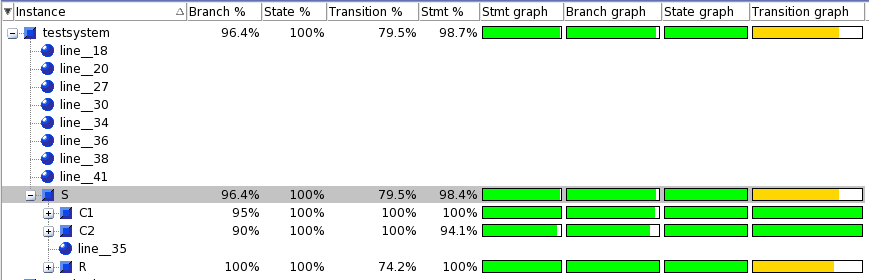
\includegraphics[scale=0.7]{PremiereCorrection/ResAfterVHD.PNG}
\caption{Rapport de couverture}

\end{figure}

\begin{figure}[!h]
\advance\leftskip+3cm
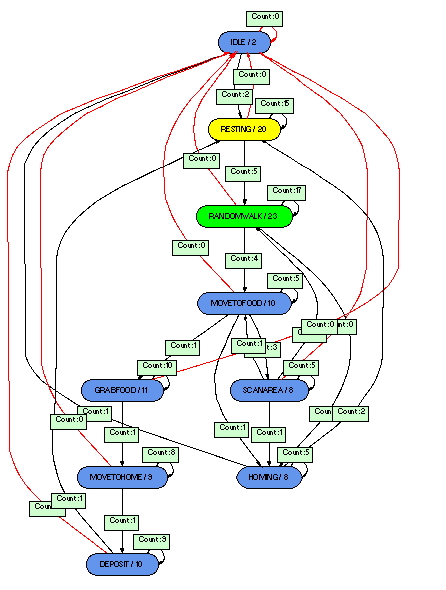
\includegraphics[scale=0.7]{PremiereCorrection/GRAPH.PNG}
\caption{Graph de couverture des états du robot}

\end{figure}


\paragraph{Interprétation des résultats}

La couverture n'est pas totales car je n'ai pas testé si le reset marche pour tout les états. De plus, les counters ne rentre pas dans les configurations permettant d'avoir un branching parfait. 
\sautligne 

Néanmoins, je ne pense pas qu'il est nécessaire d'aller plus loin. Les tests de couvertures sont passé haut la main.

\newpage


\section{Vérification d'assertions temporelles}

\section{Annexes}
\subsection{Correction de robot.vdh}
 
\end{document}